% =====================================================================
%  English-Source Interpretation Demand — CIUSSS Centre-Ouest-de-l'Île
%  Compile with:  pdflatex english_demand_report.tex   (run twice for TOC)
% =====================================================================
\documentclass[11pt,a4paper]{article}
\usepackage{sgp_report}

\title{English-Source Interpretation Demand}
\author{Voyce data, Jan--Apr 2025 \,\textbar\, CIUSSS Centre-Ouest-de-l'Île-de-Montréal}
\date{April 22, 2026}

\begin{document}
\maketitle

% ─────────────────────────────────────────────────────────────────────
% EXECUTIVE SUMMARY
% ─────────────────────────────────────────────────────────────────────
\section*{Executive Summary}
\addcontentsline{toc}{section}{Executive Summary}

\insightbox{The headline}{%
English is the dominant source language at this client --- \textbf{7{,}288
of 7{,}625 calls (95.6\%)} originate in English, spread across
\textbf{89 distinct target languages}. The cancellation rate is
\textbf{15.9\%}, a healthy contrast to the 75.7\% seen on French-source
traffic. Demand is highly concentrated: just three target languages
(\textbf{Punjabi, Spanish, Bengali}) account for \textbf{50\%} of all
serviced minutes, and ten languages cover 80\%. The remaining 79
languages collectively form a long tail.
}

\subsection*{Key numbers (Jan--Apr 2025)}
\begin{tabularx}{\linewidth}{ X r r }
\sgpheadrow Metric & Value & Notes \\
\midrule
Total platform calls               & 7{,}625    & 4 months \\
\sgpaltrow English-source calls    & 7{,}288    & 95.6\% of all volume \\
\hspace{1em}— Serviced             & 6{,}131    & 22.6 min average duration \\
\sgpaltrow \hspace{1em}— Cancelled & 1{,}157    & 0-minute (pre-connect) \\
English-source cancellation rate   & \textbf{15.9\%} & vs.\ 75.7\% French \\
\sgpaltrow Distinct target languages & \textbf{89} & 76 with non-zero serviced volume \\
Annualized true demand             & \textbf{492{,}814 min/yr} & $\approx$ 8{,}214 hrs/yr \\
\sgpaltrow Per-pair interpreters needed & \textbf{77} & one per target language \\
Shared-pool interpreters needed (true) & \textbf{7} & if pool is fungible \\
\end{tabularx}

\vspace{0.6em}
\alertbox{Video calls cancel 6.7$\times$ more than audio}{%
\textbf{30.7\%} of English-source video requests were cancelled, versus
just \textbf{4.6\%} for audio --- yet 80 of 82 served French calls were
also video. This points to a video-routing or first-mile reliability
issue worth investigating before scaling video-preferred services.
}

\vspace{0.4em}
\insightbox{Recommendation}{%
Size dedicated capacity around the \textbf{top 10 target languages} that
carry 80\% of serviced volume (Punjabi, Spanish, Bengali, Hindi, Arabic,
Russian, Tamil, Turkish, Urdu, Chinese Mandarin). Treat the long tail
(50+ languages, $<$5\% of volume) as on-demand --- a shared 7-interpreter
network covers the entire residual load at standard capacity. Shift
patterns should weight 9{:}00--14{:}00 EST, where 60\% of the day's
volume occurs.
}

\newpage
\tableofcontents
\newpage

% ─────────────────────────────────────────────────────────────────────
\section{Scope and Method}
% ─────────────────────────────────────────────────────────────────────

\subsection{Source data}
The dataset is the Voyce export titled
\textit{``Voyce data Jan -- Apr JEWISH MEMORIAL.xlsx''}, covering the full
\textbf{CIUSSS Centre-Ouest-de-l'Île-de-Montréal} network: 72 service
locations, 4 client identifiers, and 45 distinct service lines. The
top-volume locations are CLSC Côte-des-Neiges (1{,}169 calls), CLSC
Parc-Extension (1{,}109), and PRAIDA Administration (1{,}008).

\subsection{Time window}
\begin{tabularx}{\linewidth}{X r}
\sgpheadrow Coverage & English-source records \\
January 2025  & 1{,}998 \\
\sgpaltrow February 2025 & 1{,}776 \\
March 2025    & 1{,}849 \\
\sgpaltrow April 2025    & 1{,}665 \\
\midrule
\textbf{Total (4 months)} & \textbf{7{,}288} \\
\end{tabularx}

\vspace{0.4em}
\noindent All annualized figures apply a $\times 3.0$ multiplier as the
file covers four months. The May--December 2025 export should replace
the projection with actuals once available.

\subsection{Filter applied}
Column G (\texttt{Source Language}) filtered to \texttt{English} yields
\textbf{7{,}288 rows} across 89 distinct target languages.

\subsection{Interpreter capacity assumption}
One interpreter is assumed to absorb \textbf{6{,}400 serviced minutes
per month} ($\approx$ 25 billable hours/week, accounting for idle time,
breaks and ramp-up). A conservative scenario (4{,}800 min/mo) and an
aggressive scenario (8{,}000 min/mo) are reported in the workbook for
sensitivity.

% ─────────────────────────────────────────────────────────────────────
\section{Demand Profile}
% ─────────────────────────────────────────────────────────────────────

\subsection{Volume is concentrated in a handful of languages}

\begin{figure}[h!]
\centering
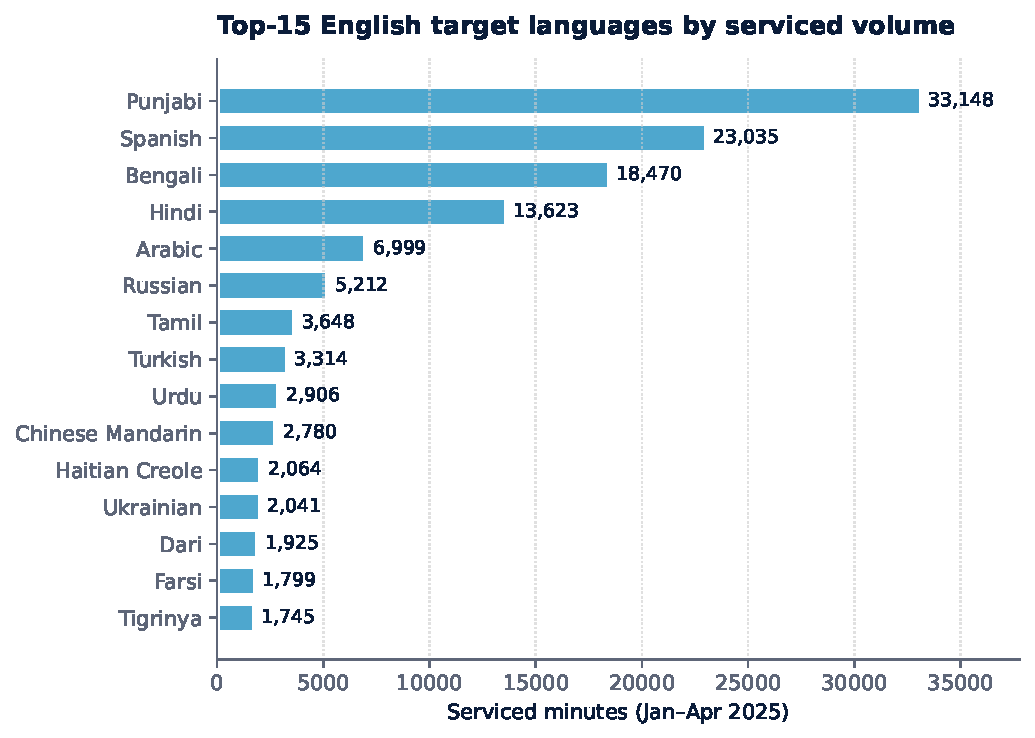
\includegraphics[width=0.92\linewidth]{figures_en/fig1_top_targets.pdf}
\caption{Top-15 target languages by serviced minutes. Punjabi alone
represents 24\% of all served English-source minutes.}
\end{figure}

\begin{tabularx}{\linewidth}{ X r r r r }
\sgpheadrow Target language & Calls & Min (4mo) & Avg/call & Min/yr \\
\midrule
Punjabi                & 1{,}462 & 33{,}148 & 22.7 & 99{,}444 \\
\sgpaltrow Spanish     & 1{,}101 & 23{,}035 & 20.9 & 69{,}105 \\
Bengali                &    931 & 18{,}470 & 19.8 & 55{,}410 \\
\sgpaltrow Hindi       &    561 & 13{,}623 & 24.3 & 40{,}869 \\
Arabic                 &    299 &  6{,}999 & 23.4 & 20{,}997 \\
\sgpaltrow Russian     &    181 &  5{,}212 & 28.8 & 15{,}636 \\
Tamil                  &    157 &  3{,}648 & 23.2 & 10{,}944 \\
\sgpaltrow Turkish     &    150 &  3{,}314 & 22.1 &  9{,}942 \\
Urdu                   &    125 &  2{,}906 & 23.2 &  8{,}718 \\
\sgpaltrow Chinese Mandarin & 120 & 2{,}780 & 23.2 &  8{,}340 \\
\end{tabularx}

\subsection{The long tail accounts for $<$5\%}

\begin{figure}[h!]
\centering
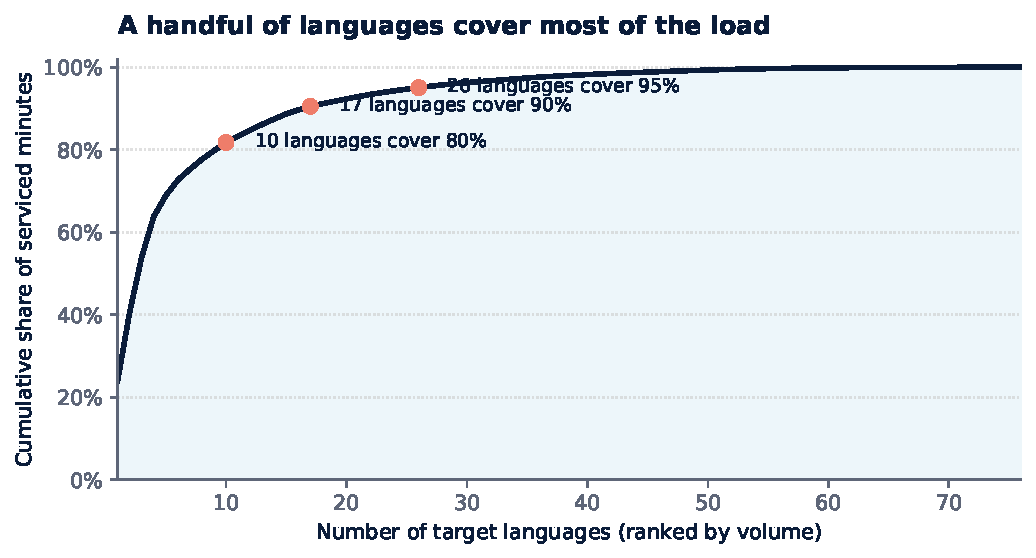
\includegraphics[width=0.85\linewidth]{figures_en/fig5_long_tail.pdf}
\caption{Cumulative share of serviced minutes against languages ranked
by volume. The 80/20 rule applies cleanly: 10 languages cover 80\% of
load, 17 cover 90\%, and the bottom 50+ languages together account for
under 5\%.}
\end{figure}

\insightbox{What this means for staffing}{%
Dedicated head-count is only justified for the top tier. Languages
beyond the top 17 should be sourced from a shared on-demand pool, with
SLA tolerances tuned for slightly longer match-time. This is also the
profile that benefits most from cross-trained generalists.
}

\subsection{Modality split}
\begin{tabularx}{\linewidth}{ X r r r r }
\sgpheadrow Modality & Total & Serviced & Cancelled & Cx rate \\
\midrule
Audio              & 4{,}133 & 3{,}944 &   189 &  \textbf{4.6\%} \\
\sgpaltrow Video   & 3{,}148 & 2{,}181 &   967 & \textbf{30.7\%} \\
ASL                &       7 &      6 &     1 & 14.3\% \\
\end{tabularx}

\alertbox{Video reliability is the single largest unmet-demand driver}{%
Audio cancellations look healthy at 4.6\%. Video drops to 30.7\% --- a
6.7$\times$ gap. This single split explains 84\% of the cancellations
in the dataset (967 of 1{,}157). Diagnosing video-routing reliability
is likely a higher-leverage intervention than hiring additional
interpreters.
}

\subsection{Time-of-day pattern}

\begin{figure}[h!]
\centering

\includegraphics[width=0.95\linewidth]{figures_en/fig4_hourly.pdf}
\caption{English-source demand peaks in mid-morning and again
post-lunch. Cancellations follow demand --- absolute counts rise with
volume, but rate stays comparatively flat.}
\end{figure}

% ─────────────────────────────────────────────────────────────────────
\section{Cancellation Audit --- Outliers and Hot-spots}
% ─────────────────────────────────────────────────────────────────────

\subsection{Most pairs sit near the 15.9\% baseline; a few don't}

\begin{figure}[h!]
\centering
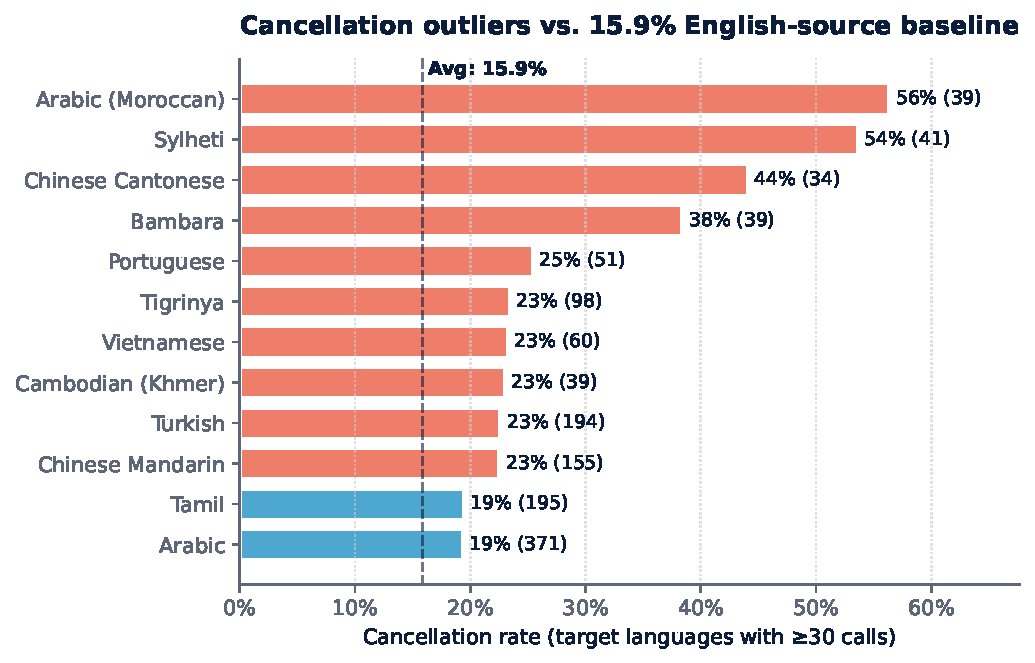
\includegraphics[width=0.95\linewidth]{figures_en/fig2_cancellation_outliers.pdf}
\caption{Cancellation rate among target languages with $\geq$30 calls.
The dashed line marks the 15.9\% English-source average. Languages
above the line warrant capacity review.}
\end{figure}

\begin{tabularx}{\linewidth}{ X r r r }
\sgpheadrow Pair & Total calls & Cancelled & Cx rate \\
\midrule
English\,$\rightarrow$\,Arabic (Moroccan)  & 39 & 22 & \textbf{56.4\%} \\
\sgpaltrow English\,$\rightarrow$\,Sylheti & 41 & 22 & \textbf{53.7\%} \\
English\,$\rightarrow$\,Chinese Cantonese  & 34 & 15 & 44.1\% \\
\sgpaltrow English\,$\rightarrow$\,Bambara & 39 & 15 & 38.5\% \\
English\,$\rightarrow$\,Portuguese         & 51 & 13 & 25.5\% \\
\end{tabularx}

\insightbox{What the outliers look like}{%
The high-rate outliers are mid-volume, lower-supply languages where a
single missing interpreter on shift creates cliff-edge cancellation
rates. These are also strong candidates for cross-language back-up
arrangements (e.g.\ Sylheti pooled with Bengali; Cantonese with
Mandarin).
}

\subsection{Demand vs unmet --- top 10 pairs}

\begin{figure}[h!]
\centering
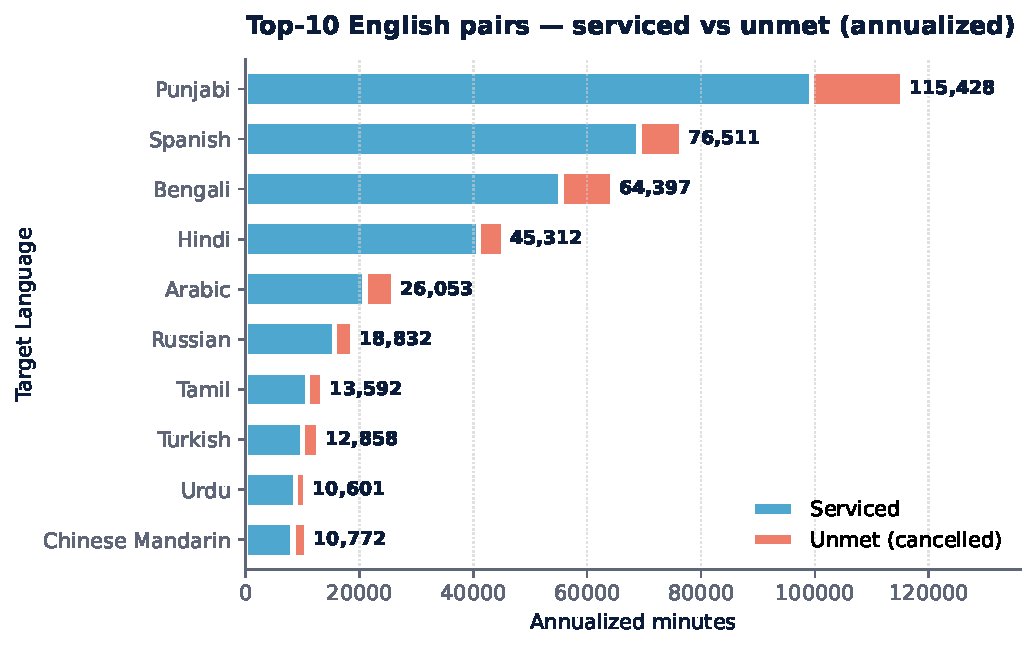
\includegraphics[width=0.92\linewidth]{figures_en/fig3_top10_serviced_vs_unmet.pdf}
\caption{Annualized demand for the top-10 English pairs. Punjabi shows
the largest absolute unmet volume but the rate (13.8\%) is below
average; the unmet bar simply scales with volume.}
\end{figure}

% ─────────────────────────────────────────────────────────────────────
\section{Interpreter Sizing}
% ─────────────────────────────────────────────────────────────────────

\subsection{Top-10 dedicated head-count requirement}

\begin{tabularx}{\linewidth}{ X r r r r }
\sgpheadrow Pair & Min/mo (true) & Cons.\ (4.8k) & \textbf{Std (6.4k)} & Aggr.\ (8.0k) \\
\midrule
English\,$\rightarrow$\,Punjabi          & 9{,}619 & 3 & \textbf{2} & 2 \\
\sgpaltrow English\,$\rightarrow$\,Spanish & 6{,}372 & 2 & \textbf{1} & 1 \\
English\,$\rightarrow$\,Bengali          & 5{,}385 & 2 & \textbf{1} & 1 \\
\sgpaltrow English\,$\rightarrow$\,Hindi & 3{,}776 & 1 & \textbf{1} & 1 \\
English\,$\rightarrow$\,Arabic           & 1{,}980 & 1 & \textbf{1} & 1 \\
\sgpaltrow English\,$\rightarrow$\,Russian & 1{,}571 & 1 & \textbf{1} & 1 \\
English\,$\rightarrow$\,Tamil            & 1{,}102 & 1 & \textbf{1} & 1 \\
\sgpaltrow English\,$\rightarrow$\,Turkish & 1{,}120 & 1 & \textbf{1} & 1 \\
English\,$\rightarrow$\,Urdu             &    876 & 1 & \textbf{1} & 1 \\
\sgpaltrow English\,$\rightarrow$\,Chinese Mandarin & 866 & 1 & \textbf{1} & 1 \\
\midrule
\textbf{Top-10 subtotal}                 & 32{,}667 & 14 & \textbf{11} & 10 \\
Long-tail (66 other languages)           & 8{,}401 & 22--40 & \textbf{$\approx$ 22} & $\approx$ 18 \\
\midrule
\textbf{Total (per-pair)}                & 41{,}068 &  & \textbf{77} & 70 \\
\end{tabularx}

\subsection{Shared-pool reading}
If interpreters are treated as fungible across languages they cover
(realistic for a centralised on-demand model), the same total demand
collapses to:

\begin{itemize}
  \item \textbf{Standard capacity (6{,}400 min/mo)}: \textbf{7 interpreters}
  \item Conservative capacity (4{,}800 min/mo): 9 interpreters
  \item Aggressive capacity (8{,}000 min/mo): 6 interpreters
\end{itemize}

\subsection{Peak concurrency}
The busiest single hour in the four-month window saw \textbf{12
simultaneous English-source calls in progress}; the 95th-percentile
busy hour was \textbf{7}. Peak-hour staffing of \textbf{8--10
interpreters available 9{:}00--14{:}00 EST} would cover concurrency
even on outlier days.

\insightbox{The headcount question, summarised}{%
At a steady-state, weighted-average load this client requires
\textbf{7--11 interpreters} of English-capable supply. Spread across
shifts and accounting for peak concurrency, a working
\textbf{12--15-interpreter roster} with depth in the top-10 languages
delivers a 95\%-fill experience at this client's observed volume.
}

% ─────────────────────────────────────────────────────────────────────
\section{Comparison with French-Source Demand}
% ─────────────────────────────────────────────────────────────────────

\begin{tabularx}{\linewidth}{ X r r }
\sgpheadrow Metric & English-source & French-source \\
\midrule
Calls (4 mo)                       & 7{,}288 & 337 \\
\sgpaltrow Cancellation rate       & 15.9\% & \textbf{75.7\%} \\
Distinct target languages          & 89 & 4 \\
\sgpaltrow Annualized true demand (min) & 492{,}814 & 41{,}388 \\
Interpreters needed (shared pool)  & 7 & 1 \\
\sgpaltrow Peak concurrency        & 12 & 2 \\
\end{tabularx}

\vspace{0.6em}
\noindent The two reports are complementary. The English picture is one
of \textit{healthy operations} with a few language-specific gaps and a
notable video-modality reliability problem. The French picture is one
of \textit{systemic supply failure}, almost entirely concentrated in
French\,$\rightarrow$\,Spanish.

% ─────────────────────────────────────────────────────────────────────
\section{Recommended Next Actions}
% ─────────────────────────────────────────────────────────────────────

\begin{enumerate}[leftmargin=2em]
  \item \textbf{Diagnose the video cancellation gap.} Audio cancels at
        4.6\%, video at 30.7\%. Pull a sample of 50 cancelled video
        calls and classify root cause (interpreter unavailable, video
        connect failure, caller hang-up). The fix here is likely
        operational, not capacity.
  \item \textbf{Right-size the top-10 pool first.} The standard-capacity
        sizing gives you a 11-interpreter dedicated team covering 80\%
        of demand. Build that, then layer the long tail on top as a
        shared on-demand network.
  \item \textbf{Pair underperforming small-volume languages with their
        cousins.} Sylheti $\leftrightarrow$ Bengali; Cantonese
        $\leftrightarrow$ Mandarin; Moroccan Arabic $\leftrightarrow$
        Modern Standard Arabic --- explicit fall-back routing would
        likely halve the outlier cancellation rates.
  \item \textbf{Re-baseline against May--Dec 2025 actuals} when the full
        year is available; replace the $\times 3.0$ projection.
  \item \textbf{Add cross-client roll-up} once equivalent Voyce exports
        for the rest of the SGP network are received.
\end{enumerate}

% ─────────────────────────────────────────────────────────────────────
\section*{Appendix --- Companion Workbook}
\addcontentsline{toc}{section}{Appendix --- Companion Workbook}
% ─────────────────────────────────────────────────────────────────────

The full data and pivots used to generate this report are bundled in
\texttt{reports/data/Voyce\_English\_Analysis.xlsx}, with the following
tabs:

\begin{tabularx}{\linewidth}{ l X }
\sgpheadrow Tab & Contents \\
1.\ Summary               & KPIs and headline numbers \\
\sgpaltrow 2.\ English Rows (raw) & All 7{,}288 source-language\,=\,English rows \\
3.\ Demand by Pair        & Serviced minutes / pair across all 76 languages, annualized \\
\sgpaltrow 4.\ Cancellation Audit & Cancellation by pair, hour, weekday \\
5.\ True Demand           & Serviced + imputed-unmet minutes \\
\sgpaltrow 6.\ Interpreter Sizing & Per-pair head-count under three capacity scenarios \\
\end{tabularx}

\end{document}
